\label{chapter:Avaliacao}

\par
\textcolor{red}{Nesta seção será apresentado os processos e avaliações dos testes do projeto, com intuito de expor se os modelos de classificação e associação foram bem sucedidos, se a taxa de precisão da classificação alcançou a porcentagem do que se era esperado, se foi gerado as regras que eram necessarias para a avaliação dos dois modelos e entre outros.}

\par
\textcolor{red}{Para a avaliação do experimento, no processo de mineração, foi utilizado um notebook pessoal da marca DELL do modelo Inspiron 5558, que possui um processador Intel(R) Core(TM) i5-5200U CPU @ 2.20 GHz com uma mémoria instalada de 16 GB. Para o uso dos algoritmos de classificação e associação para mineração e avaliação, foi utilizado a versão estável 3.8.3 do software WEKA.}

\section{Avaliando Com o Algoritmo J48}

\par
\textcolor{red}{De forma para validar o modelo feito pela atividade de classificação, foi utilizada um filtro do Explore do WEKA chamado de \textit{RemovePercentage} para poder fazer a separação da base de dados para treinamento e teste. Possuindo 1.574 registros, a base de dados foi separada em duas partes, tendo como 70\% dos dados para treinamento com 1086 instancias e 30\% dos dados para teste com 486 instancias. Após o processo de utilizar o modelo de classificação do conjunto de treinamento para testar no conjunto de teste, o algoritmo J48 obteve como resultado uma precisão de 57\% das instâncias classificadas corretamente e de aproximadamente 43\% das instancias classificada incorretamente, como demonstrado na Figura 31.}

\par
\begin{figure}[!htp]
	\begin{center}
    \caption{\label{fig:waveform_fig} Resultado de acurácia do modelo de validação.}
	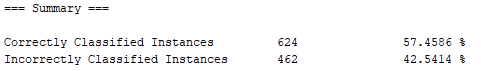
\includegraphics[scale=0.99]{Figuras/Modelo_de_validacao.png}
	\end{center}
    \legend{Fonte: Próprio autor.}
\end{figure}

\par
\textcolor{red}{Na base de dados balanceada, através do software WEKA, á análise por arvore de decisão foi feita utilizando o algoritmo J48, usando a opção \textit{cross-validation} para a sua execução, com um valor para fold igual a dez e com a variável dependente Aprovado. A árvore de decisão foi capaz de identificar corretamente aproximadamente 53\% instâncias das 1.574 inseridas, como apresentado na Figura 32. Pode se notar que a taxa de acurácia obtida pelo algoritmo tem um valor aproximado da taxa do modelo de validação que foi mencionado, comprovando dessa forma que o modelo avaliado é considerado útil para ser utilizado.}

\par
\begin{figure}[!htp]
	\begin{center}
    \caption{\label{fig:waveform_fig} Resultado de acurácia do modelo de base de dados.}
	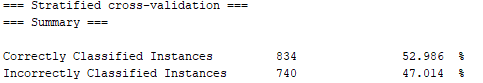
\includegraphics[scale=0.99]{Figuras/Resultado_acuracia.png}
	\end{center}
    \legend{Fonte: Próprio autor.}
\end{figure}

\par
\textcolor{red}{Na Figura 33 são apresentados os valores de acurácia para cada classe do atributo Aprovado. Pode-se notar que os valores de precisão apresentam resultados semelhantes para as classes Sim e Nao, com taxa acima dos 50\% e abaixo dos 70\% de precisão.}

\par
\begin{figure}[!htp]
	\begin{center}
    \caption{\label{fig:waveform_fig} Detalhes da acurácia das classes.}
	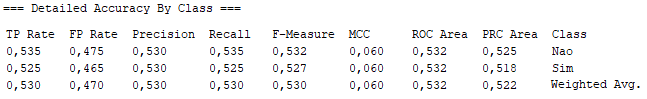
\includegraphics[scale=0.93]{Figuras/Tabela_de_acuracia_das_classes.png}
	\end{center}
    \legend{Fonte: Próprio autor.}
\end{figure}

\textcolor{red}{A Figura 34, que apresenta matriz de classificação para cada classe, indica que, na classe Nao, de 779 ocorrências, apenas 366 registros foram classificados corretamente, enquanto na classe Sim, de 795 ocorrências, apenas 374 registros foram classificados corretamente.}

\par
\begin{figure}[!htp]
	\begin{center}
    \caption{\label{fig:waveform_fig} Matriz de confusão.}
	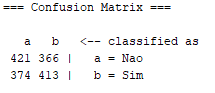
\includegraphics[scale=0.99]{Figuras/Matriz_de_classificacao.png}
	\end{center}
    \legend{Fonte: Próprio autor.}
\end{figure}

\par
\textcolor{red}{Podemos notar que a taxa de acurácia do modelo utilizado, deu como resultado aproximadamente 53\% de instancias classificadas corretamente, um valor um pouco abaixo do que esperado, que era de 70\% de precisão para ser um bom modelo. Como foi explicado durante a preparação do modelo, que foi necessário utilizar técnicas para balancear os dados com o intuito de resolver o problema de classe rara, teve como consequência, uma queda drástica da quantidade de registros, onde, de 8.571 registros caiu para 1.574 registros balanceados. Por causa desse balanceamento, foi um dos fatores que motivaram para que o modelo não possuísse registros suficiente a fim de obter uma taxa razoável  de instâncias classificadas corretamente.}



\section{Avaliando Com o Algoritmo Apriori}


\textcolor{red}{Para a mesma base de dados, foi realizado outra análise utilizando o algoritmo de associação Apriori, tendo como as parametrizações de suporte e confiança mínimos na geração das regras que sejam mais relevantes, para os resultados esperados associada a variável Aprovado. Para o suporte e confiança mínima para avaliação, foi utilizado como base a porcentagem usada no trabalho de \citeonline{LeandroSilva2014}, que foi feito testes com 50\%, 30\%, 25\% e 15\% de suporte geração dos items set e 70\% de confiança na geração de regras para todos os casos de suporte avaliados.}

\par
\textcolor{red}{Para os testes, foi utilizado toda a base de dados com um total de 8571 registros. Na janela de configuração do algoritmo Apriori apresentado na Figura 35, foi definido para a quantidade máxima de regras geradas foi colocado na opção \textit{numRules} o número 100 para todos os teste, logo acima, no parâmetro \textit{metricType} a métrica utilizada nos testes foi a de confiança tendo a sua taxa como 70\% para as regras geradas, e para os limites inferiores (\textit{lowerBoundMinSupport}) e superiores (\textit{upperBoundMinSupport}) mínimo de suporte é a opção que é definido a taxa de porcentagem mínima do suporte.}


\par
\begin{figure}[!htp]
	\begin{center}
    \caption{\label{fig:waveform_fig} Janela de configuração do algoritmo Apriori.}
	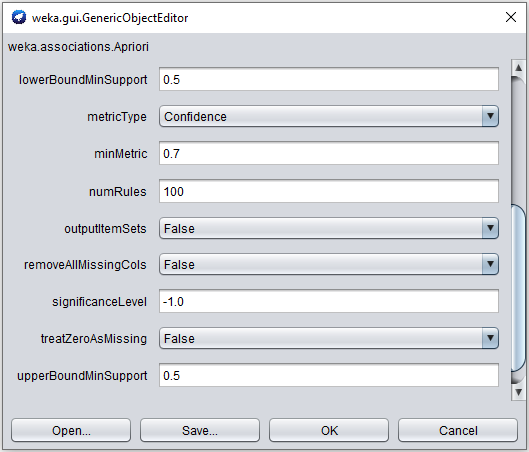
\includegraphics[scale=0.70]{Figuras/Janela_configuracao_apriori.png}
	\end{center}
    \legend{Fonte: Próprio autor.}
\end{figure}


\par
\textcolor{red}{Nos primeiros testes foi observado que independentemente da taxa de suporte, todas regras geradas para aprovados, tem uma forte tendência a ter a classe Nao como resultado, segundo \citeonline{Amaral2016}, isso acontece pelo fato de existe uma maior quantidade de um registro do que outro, fazendo com que o algoritmo tende a gerar regras somente para a maior quantidade fornecida, isto é, pegando como exemplo a base de dados utilizada que possui  91\% dos registros de candidatos que não foram aprovados e 9\% de candidatos que foram aprovados, o algoritmo só vai gerar regras para os candidatos que não foram aprovados. No trabalho de \citeonline{LeandroSilva2014} não ocorreu esse mesmo problema, pelo fato de o modelo dele possuir 4 classes com registros bem divididos para sua variável Nota.}


\par
\textcolor{red}{No intuito de resolver esse tipo de problema, para que ele possa gerar as melhores regras para ambas as classes, foi feita a separação da base em 2 partes, uma base com os candidatos que foram aprovados com um total de 787 registros e outra base com os candidatos que não foram aprovados com um total de 7784 registros. Após todo esse processo, foi feito os testes paras as duas bases, tendo com sucesso regras geradas para ambas as partes. Os testes foram feitos com 3 quantidades de atributos diferente, sendo que, uma foi feito com os atributos que sobraram após a remoção dos que eram desnecessários para o trabalho (22 atributos), os atributos que a seleção de atributos do WEKA selecionou como mais relevantes para a classificação (9 atributos) e o atributos que \citeonline{LeandroSilva2014} selecionaram para os testes de associação do trabalho deles (4 atributos).}

\par
\textcolor{red}{O motivo da escolha desses atributos para os testes, foi para saber os resultados que eram obtidos nos três tipos, principalmente na base com 22 atributo, saber também, se tem alguma semelhança com os resultados do trabalho de \citeonline{LeandroSilva2014} e também com os resultados obtidos com o algoritmo de classificação utilizado nesse trabalho. Na Tabela 2, apresenta as parametrizações de suporte e confiança utilizadas para o algoritmo Apriori, junto com as regras geradas paras as quatros porcentagens de suporte testadas, regras essas associada a variável Aprovado.}


\par
\begin{table}[!htp]
	\begin{center}
    \caption{\label{fig:waveform_fig} Tabela de parametros dos testes.}
	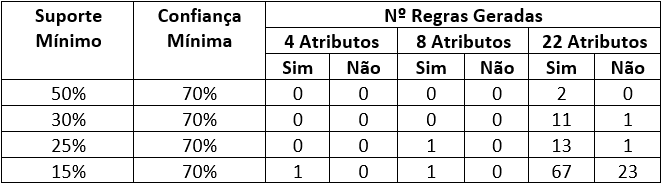
\includegraphics[scale=0.90]{Figuras/Tabela_de_parametros_apriori.png}
	\end{center}
\end{table}

\par
\textcolor{red}{Podemos notar que nas colunas de 4 atributos e 9 atributos da classe Não, para todos as porcentagens de suportes mínimos testado, nenhuma regra foi gerada, diferente da coluna de não aprovados com 22 atributos, que de três dos quatros suportes mínimos testados geraram pelo menos uma regra. Na coluna de 22 atributos para a classe Sim de aprovados, podemos obsservar que ela obteve as maiores quantidades de regras geradas para todas as taxas de suporte mínimo especificadas e que para as demais colunas da classe sim para os outros atributos, pelo menos uma regra foi gerada.}

\par
\textcolor{red}{Durantes os testes foi analisando também, que tanto para os candidatos aprovados quanto para os não aprovados, possuíam a mesma quantidade de ciclo de performance (vezes que o algoritmo foi executado) para obter as regras geradas, sendo que para o suporte de 50\% ele executou 10 vezes, 30\% executou 14 vezes, 25\% executou 15 vezes e para 15\% ele executou 17vezes. Também foi observado que durante a avaliação dos dados, para cada teste do suporte, a quantidade de itens set gerados variavam de 1 produto até no máximo 11 produtos gerados, como apresentado no exemplo da Figura 36.}


\par
\begin{figure}[!htp]
	\begin{center}
    \caption{\label{fig:waveform_fig} Exemplo dos dados com 22 atributos com suporte mínimo 15\% e confiança mínima 70\%.}
	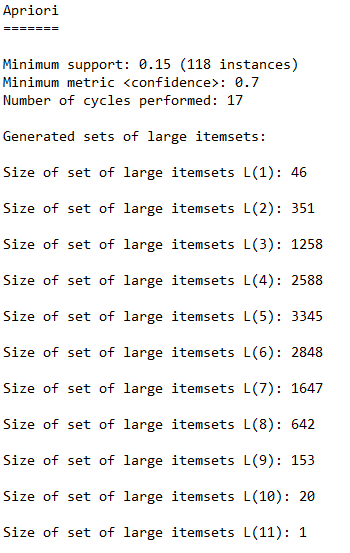
\includegraphics[scale=0.90]{Figuras/Resultados_valores_apriori.png}
	\end{center}
    \legend{Fonte: Próprio autor.}
\end{figure}

\par
\textcolor{red}{}